\section{Hypersonic compressible turbulent boundary layers and wall heat-transfer}
\label{sec:background:turbulent-boundary-layers-wall-heat-transfer}

The boundary layer is referred to as the region of flow near a viscous wall, where the bulk flow needs to decelerate down to the no-slip condition at the wall. Whole books have been dedicated to the boundary layer, i.e. Schlichting's "Boundary-Layer Theory" \cite{SchlichtingGersten2017BoundaryLayer}. Hence this section is kept to a minimum only highlighting certain aspects of the turbulent hypersonic cold-wall boundary layer, which are relevant for the later parts of this work.

\subsection{Difference in boundary layer profiles}
\label{subsec:background:wall-units}


Figures~\ref{fig:background:dns-velocity-profiles} and~\ref{fig:background:dns-temperature-profiles} show the difference in the Reynolds averaged velocity and temperature boundary layer profiles from DNS calculations of a transonic cold-wall (C09) a hypersonic near-adiabatic-wall (M6Tw076) and hypersonic cold-wall (M6Tw025) flow. The non-dimensional wall coordinate is \(y^+=y u_\tau/\nu_w\), where \(y\) is the physical wall-normal distance, \(u_\tau=\sqrt{\tau_w/\rho_w}\) is the friction velocity and \(\nu_w=\mu_w/\rho_w\) is the kinematic viscosity at the wall. Each profile is normalized by its own freestream velocity or temperature. M6Tw076 and M6Tw025 are the near-adiabatic and strongly cooled hypersonic cases of Zhang et al.~\cite{zhang2018direct}. C09 is the cooled transonic case at \(M_\infty=0.8\) of Iwatani et al.~\cite{iwatani2025subharmonic}, sampled in the fully turbulent region.
\par\medskip

While the velocity profiles of these three cases show a similar trend, the temperature boundary layer profile of the hypersonic cold-wall M6Tw025 profile has a pronounced temperature peak inside of the boundary layer. The near-adiabatic M6Tw076 case has a nearly flat near-wall temperature profile. It retains a small nonzero wall gradient and a weak interior maximum, followed by a gradual decrease towards the freestream. C09 also has a small interior maximum (Figure~\ref{fig:background:dns-temperature-profiles} inset), but with much less kinetic energy in the freestream that can be converted to internal energy when the flow is being slowed to the wall, this peak is much less severe. Thus, the strength and location of the thermal maximum distinguish these profiles. The cases differ in Reynolds number and wall thermal condition, so this comparison does not isolate the effect of Mach number or compressibility effects.

\begin{figure}[H]
    \centering
    % Figure provenance:
    % Original vector export: tmp/boundary_layer_profile_comparison/velocity_profiles.pdf
    % Generating script: tmp/boundary_layer_profile_comparison/plot_profiles.py
    % Retained source data, preprocessing and scaling checks:
    % tmp/boundary_layer_profile_comparison/raw/ and source_notes.txt
    % M6Tw076/M6Tw025: Zhang, Duan and Choudhari (2018), DOI 10.2514/1.J057296.
    % Digital files: https://tmbwg.github.io/turbmodels/Other_DNS_Data/
    % Supersonic_hypersonic_flatplate/M6Tw076_Stat.dat and M6Tw025_Stat.dat
    % C09: Iwatani, Asada and Kawai (2025), DOI 10.1016/j.ijheatfluidflow.2025.109896.
    % Digital file: https://www.klab.mech.tohoku.ac.jp/database/2025IwataniIJHFF/yprof-uTr-C09.txt
    % Station X=11; inferred velocity factor 0.8; conventional y+ from archived
    % Cf and wall density, with published Sutherland C1 approximately 0.432.
    % Copied without cropping or resizing the source PDF.
    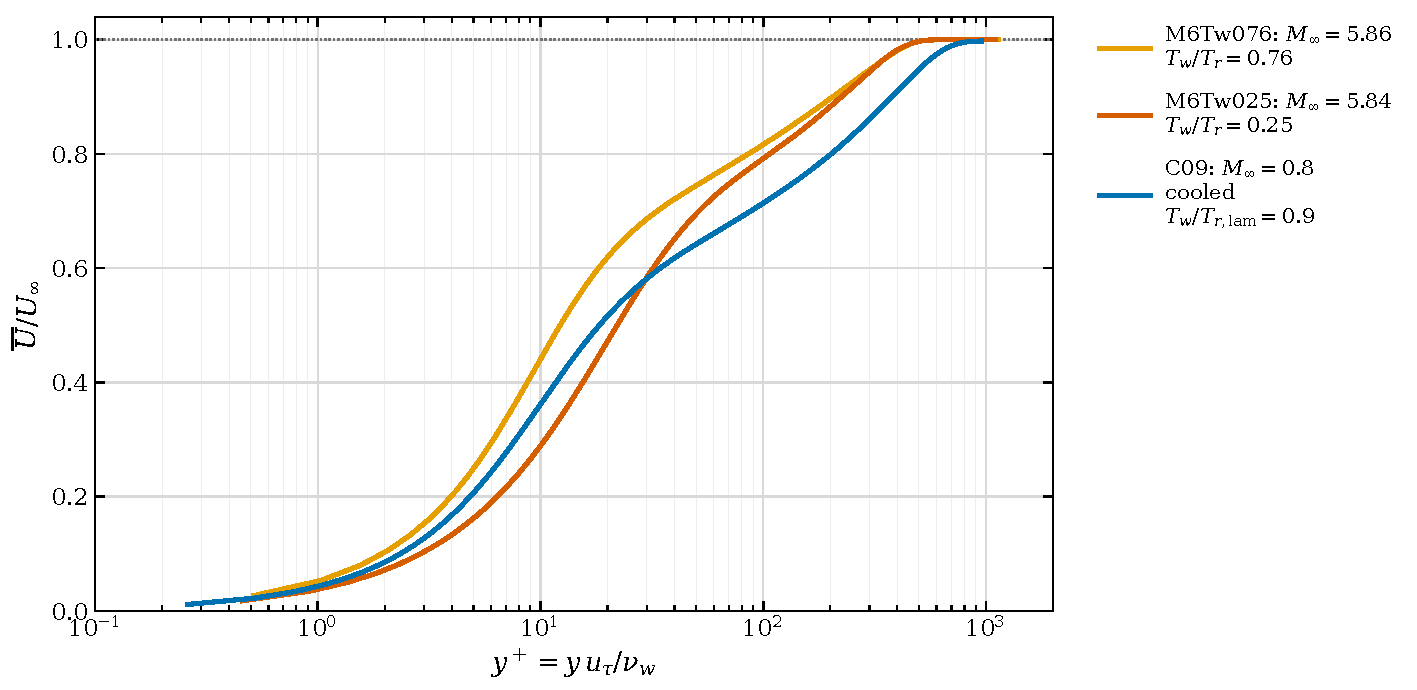
\includegraphics[width=\linewidth]{02_Background/Figures/velocity_profiles.pdf}
    \caption[DNS velocity profiles for hypersonic and subsonic turbulent boundary layers]{Freestream-normalized Reynolds-mean velocity profiles for the hypersonic M6Tw076 and M6Tw025 cases~\cite{zhang2018direct} and the fully turbulent subsonic C09 case~\cite{iwatani2025subharmonic}. All profiles use their own conventional wall units on the logarithmic \(y^+\) axis.}
    \label{fig:background:dns-velocity-profiles}
\end{figure}

\begin{figure}[H]
    \centering
    % Figure provenance:
    % Original vector export: tmp/boundary_layer_profile_comparison/temperature_profiles.pdf
    % Generating script and retained data: as for fig:background:dns-velocity-profiles.
    % Native Reynolds-mean T/Tinf columns are used for all three cases.
    % Source-sample maxima (y+, T/Tinf):
    % M6Tw025 (17.489588, 2.69037833), M6Tw076 (2.59012271, 5.46204600),
    % C09 (25.11972727, 1.02344012).
    % M6Tw076 retains the digital wall-state normalization; its discrepancy
    % from the tabulated wall temperature is discussed in the benchmark section.
    % Copied without cropping or resizing the source PDF.
    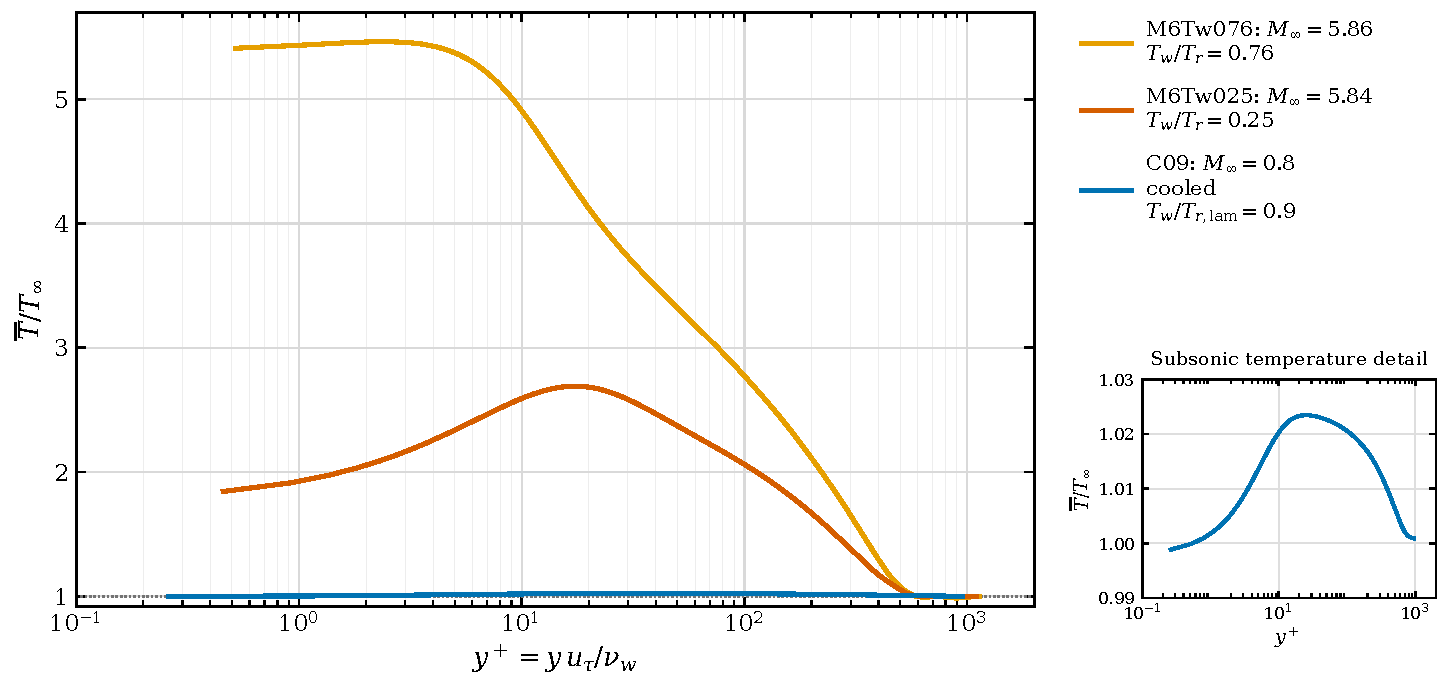
\includegraphics[width=\linewidth]{02_Background/Figures/temperature_profiles.pdf}
    \caption[DNS temperature profiles and the hypersonic cold-wall thermal maximum]{Freestream-normalized Reynolds-mean temperature profiles for the DNS cases in Figure~\ref{fig:background:dns-velocity-profiles}. The hypersonic cold-wall case M6Tw025 has a pronounced interior temperature peak, \(\overline{T}_{\max}/T_\infty\approx2.69\) at \(y^+\approx17.5\), followed by a decline towards the freestream. The near-adiabatic M6Tw076 case has only a weak near-wall maximum. The inset resolves the much smaller C09 peak, \(\overline{T}_{\max}/T_\infty\approx1.023\).}
    \label{fig:background:dns-temperature-profiles}
\end{figure}

\subsection{Compressibility and cold-wall effects and Morkovin's hypothesis}
\label{subsec:background:SRA-Morkovin}
Throughout this thesis the friction Mach number 
\begin{equation}
    M_\tau = \frac{u_\tau}{a_w},
    \qquad
    u_\tau = \sqrt{\frac{\tau_w}{\rho_w}},
\end{equation}
where \(a_w\) is the speed of sound at the wall, \(\tau_w\) the wall shear stress and \(\rho_w\) the density at the wall, is being used. The friction Mach number is discussed by Smits and Dussauge~\cite{smits2006turbulent} and is used here as an indicator for intrinsic compressibility effects, following Hasan et al.~\cite{hasan2025intrinsic}.
\par\medskip

To indicate the strength of the cold-wall effects in the used DNS references either the dimensionless wall heat-transfer rate
\begin{equation}
    B_q = \frac{q_w}{\rho_w c_p u_\tau T_w},
    \qquad
    u_\tau = \sqrt{\frac{\tau_w}{\rho_w}},
\end{equation}
with the wall heat-flux \(q_w\), wall shear stress \(\tau_w\) and heat capacity at constant pressure \(c_p\) is used. Or, as a simpler a-priori assessment, the ratio of isothermal wall temperature to adiabatic recovery temperature \(\frac{T_w}{T_r}\), e.g. \cite{zhang2018direct}.
\par\medskip

A detailed discussion of compressibility effects is beyond the scope of this work, the reader is referred to Pecnik and Hasan~\cite{pecnik2026turbulence}. Morkovin's hypothesis ~\cite{morkovin1962effects} provides a physical rationale for extending such models to compressible flow: when intrinsic compressibility effects are sufficiently small, much of the change in turbulence can be accounted for through mean-property variations \cite{fu2019turbulence}. The reference DNS studies used for assessing the turbulence models (see Section~\ref{sec:evaluation:benchmark-cases}) provide substantial support for this approximate similarity under the investigated conditions. Furthermore, the classical strong Reynolds analogy (SRA) introduces additional assumptions concerning temperature fluctuations \cite{huang2005direct}. Modified forms, including HSRA, accommodate departures from the classical relations and show approximate agreement over much of the outer boundary layer. These findings support assessing standard SA and SST formulations as compressible-flow models, but do not establish the accuracy of their momentum and thermal closures, particularly near strongly cooled walls.

\subsection{Conclusion and implications to thesis work}

The pronounced thermal-profile differences in the investigated hypersonic cold-wall case have important implications for wall-function mesh design (Section~\ref{subsec:comparative:zpg:mesh-criterion}). The linear-\(y^+\) profiles in Figures~\ref{fig:WF:dns-velocity-profiles-linear} and~\ref{fig:WF:dns-temperature-profiles-linear} relate these profile shapes to finite wall-normal spacing, because \(y^+\) is proportional to physical wall distance within each case. For wall-resolved calculations, the relevant issue is variation of the temperature gradient across the wall-to-first-cell distance: a steep but linear profile would still give an exact secant approximation to the wall derivative. Section~\ref{sec:evaluation:mesh-families-yplus} establishes the first-cell acoustic-Reynolds-number guideline through mesh-convergence studies for the investigated cases.